
% --------------------------------------------------------------- CONFIGURATIONS

\documentclass[a4paper,12pt,final,oneside]{book}

\usepackage{rapport}


% -------------------------------------------------------------- META: CONSTANTS

\newcommand{\reporttitle}{Data Mining}
\newcommand{\enseignants}{Jean-Francois~\textsc{Boulicaut}\\ Mehdi~\textsc{Kaytoue}}
\newcommand{\reportauthor}{Guillaume~\textsc{Abadie}\\ Ahmed~\textsc{Kachkach}}
\newcommand{\reportsubject}{Livrable de projet}
\newcommand{\stagetopic}{D\'ecouverte de points d'int\'er\^ets}
\newcommand{\dateperiod}{du 24 fevrier au 10 mars 2014}
\newcommand{\HRule}{\rule{\linewidth}{0.5mm}}
\setlength{\parskip}{1ex} % Espace entre les paragraphes

\hypersetup{
	pdftitle={\reporttitle},%
		pdfauthor={\reportauthor},%
		pdfsubject={\reportsubject},%
		pdfkeywords={INSA Lyon} {Data Mining}
}

\title{\reporttitle}
\author{\reportauthor}
%\setcounter{tocdepth}{4}


% ------------------------------------------------------------------------- FILE

\begin{document}


    % ------------------------------------------------------------------- HEADER

	\renewcommand{\chaptername}{} %\renewcommand{\thechapter}{}
	\renewcommand{\contentsname}{Sommaire}

	\pagestyle{empty}
	\pagenumbering{Roman}


    % ------------------------------------------------------------ HEADER: TITLE

	% Inspiré de http://en.wikibooks.org/wiki/LaTeX/Title_Creation
\begin{center}
	\begin{minipage}[t]{0.48\textwidth}
	  \begin{flushleft}
	    
\includegraphics [width=40mm]{images/logo_INSA.png} \\[0.5cm]
			INSA Lyon\\
			20, avenue Albert Einstein\\
			69621 Villeurbanne Cedex
	  \end{flushleft}
	\end{minipage}
	\begin{minipage}[t]{0.48\textwidth}
	  \begin{flushright}
	  \end{flushright}
	\end{minipage} \\[2cm]

	\textsc{\Large \reportsubject}\\[0.3cm]
	\HRule \\[0.4cm]
	{\Huge \bfseries \reporttitle}\\[0.3cm]
	{\LARGE \bfseries «~\stagetopic~»}\\[0.3cm]
	{\Large \dateperiod}\\[0.4cm]
	\HRule \\[1cm]

	
\includegraphics [scale=0.35]{images/quartz.png} \\[0.7cm]
	\begin{minipage}[t]{0.4\textwidth}
	  \begin{flushleft} \large
	    \emph{Binôme~:}\\
	    \small \reportauthor
	  \end{flushleft}
	\end{minipage}
	\begin{minipage}[t]{0.5\textwidth}
	  \begin{flushright} \large
	    \emph{Enseignants~:} \\
	    \enseignants
	  \end{flushright}
	\end{minipage}

	\vfill
	\footnotesize{Année scolaire 2013-2014}
\end{center}



    % --------------------------------------------------- HEADER: CONFIGURATIONS

	\sloppy          % Justification moins stricte : des mots ne dépasseront pas des paragraphes

    \frontmatter
		\pagestyle{empty}
		\tableofcontents
		\addtocontents{toc}{\protect\thispagestyle{empty}}

	\mainmatter
	\pagestyle{headings}

	\renewcommand{\chaptermark}[1]{\markboth{\MakeUppercase{\chaptername\ \thechapter.\ #1}}{}}
	\renewcommand{\sectionmark}[1]{\markright{\thesection{} #1}}


    % ------------------------------------------------------------------ CONTENT

    \chapter{Application}

   % TODO : Rajouter + de texte autour du contexte de ce projet, et sur les technologies utilisées dans cette première partie : Knime, ..%
    But~: trouver des points d’intérêts.

\section{Familiarisation avec les données}
    % TODO : Rajouter + de détails => format des données, origine, contexte, colonnes du CSV, ... %
    Découverte des colonnes disponibles, de leur type (attendu)
    Nous choisissons d'éliminer les données concernant la date d'upload (la date de prise de la photo étant plus pertinente)


	\chapter{Chargement et nettoyage des données}

\section{Prototypage et découverte des données}
    % TODO : Garder cette partie ici, ou faire un chapitre préliminaire où on %
    % parle du fait d'utiliser Knime puis de passer sur python ?              %
    Nous avons dans un premier temps utilisé Knime pour exploiter la base de données,
    et tester les algorithmes des clustering.

    Pour cela, nous avons d'abord configuré le nœud de lecture de fichiers CSV~: choix du
    séparateur de colonnes (tabulation, dans notre cas), autorisation des \textit{shortlines},
    gestion des valeurs manquantes, ...

\section{Types des données}
    Nous avions des types parasites dans les données. En effet nous
    avions des colonnes considérées comme ``String'' alors qu'elles étaient
    censées être des ``Double''. Ceci est dû à des valeurs parasites (la fameuse
    valeur de latitude ``trolilol'', notamment).

\section{Unicité des valeurs}
    Nous avions aussi détecté des problèmes d'unicité des valeurs. Par
    exemple, il apparaît que l'ID des photos n'est pas unique.
    Ceci peut être dû au fait que la récupération (\textit{scrapping}) de telles données
    se fait souvent de manière parallélisée, et qu'une même photo peut ainsi être récupérées plusieurs fois.

    En partant de l'hypothèse que ces duplicatas représentent les mêmes
    informations, on peut arbitrairement garder un élément par id de photo.

    Une deuxième solution, plus rigoureuse, est de créer un nouvel id garantissant
    l'unicité des informations (c'est à dire l'ensemble des colonnes pertinentes: id de
    la photo, id de l'utilisateur, date, tags et légende). C'est cette solution que nous avons choisi d'appliquer.

\section{Validité des données}
    L'élimination des duplicatas et la vérification du type des données ne suffit pas à garantir la validité de ces dernières.

    Par exemple, bien que l'année de prise d'une photo soit un entier, il est bien possible que
    celle ci soit incohérente (pour de multiples raisons: corruption de données, troll d'enseignants, etc.) et
    altère la valorisation des données (par exemple en perturbant le clustering).

    Par exemple une photo prise en 1780, avant l'invention de l'appareil photo ou
    bien une photo ayant été prise... dans 10 ans !

    Ces valeurs incohérentes peuvent parfois être conservées, ou être ``corrigées'' en les remplaçant par une moyenne globale (ou locale,
    calculée sur les éléments semblables). Dans notre cas, nous avons choisi d'éliminer les photos présentant des incohérences au vu de
    l'amplitude de celles ci, et du faible nombre de photos concernées.

    Voici les critères de validité retenus~:

    \subsection{Année de la prise de la photo}
        Ainsi, nous avons décidé de filtrer tout les photos ayant été prises
        avant l'an 2000 ou dans le futur.

        \begin{figure}[h]
            \centering
            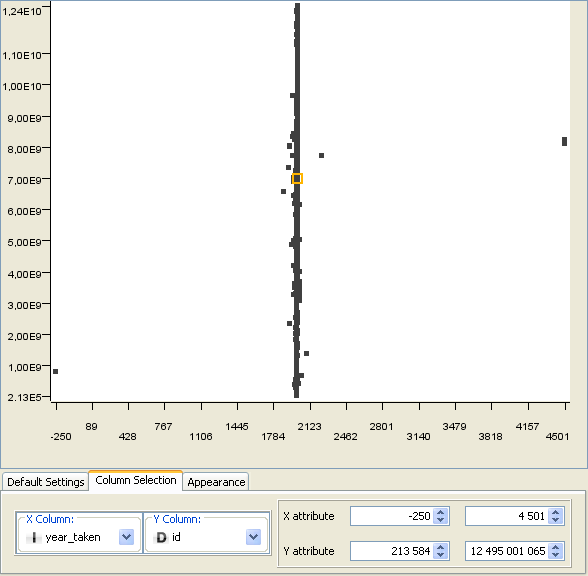
\includegraphics[scale=0.35]{../screenshots/year_id_before.png}
            \caption{données avant filtrage}
            \label{diagram:year_id_before}
        \end{figure}

        \begin{figure}[h]
            \centering
            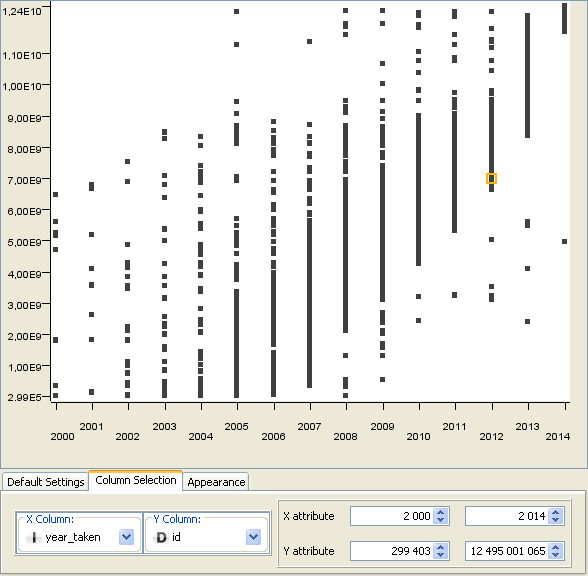
\includegraphics[scale=0.35]{../screenshots/year_id_after.png}
            \caption{données apr\`es filtrage}
            \label{diagram:year_id_after}
        \end{figure}

    \pagebreak
    \subsection{Mois et jour}

        Nous n'avons pas poussé la validation jusqu'à vérifier que la chaque jour ne dépassait pas la longueur de chaque mois, mais nous avons décidé d'éliminer toutes les photos prises à un jour > 31 (ou < 1) et les mois > 12 (ou < 1).

        \begin{figure}[h]
            \centering
            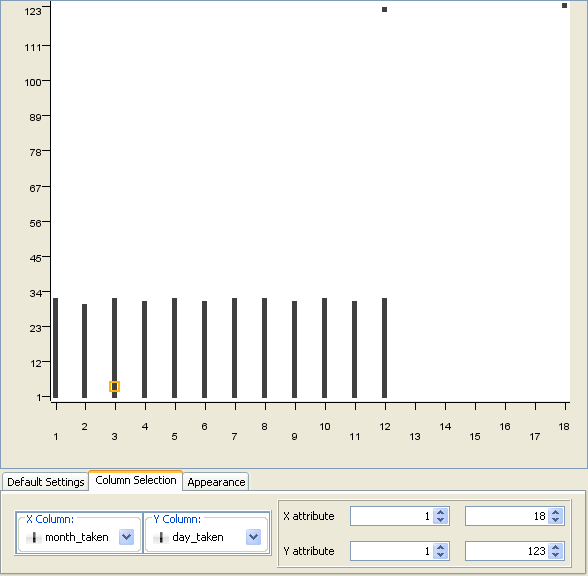
\includegraphics[scale=0.35]{../screenshots/month_day_before.png}
            \caption{données avant filtrage}
            \label{diagram:month_day_before}
        \end{figure}

        \begin{figure}[h]
            \centering
            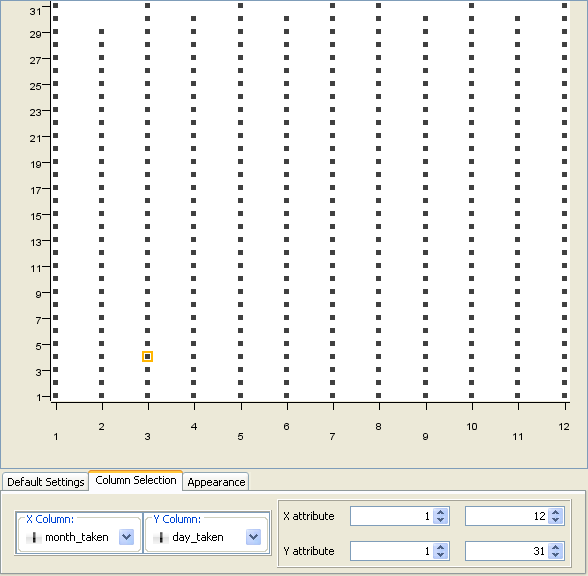
\includegraphics[scale=0.35]{../screenshots/month_day_after.png}
            \caption{données apr\`es filtrage}
            \label{diagram:month_day_after}
        \end{figure}

    \pagebreak
    \subsection{Jour et heure}

        On aimerait tous que les jours fassent plus de 24 heures, mais pour ce projet là nous avons malgré tout éliminé les valeurs plus grandes que 23.

        \begin{figure}[h]
            \centering
            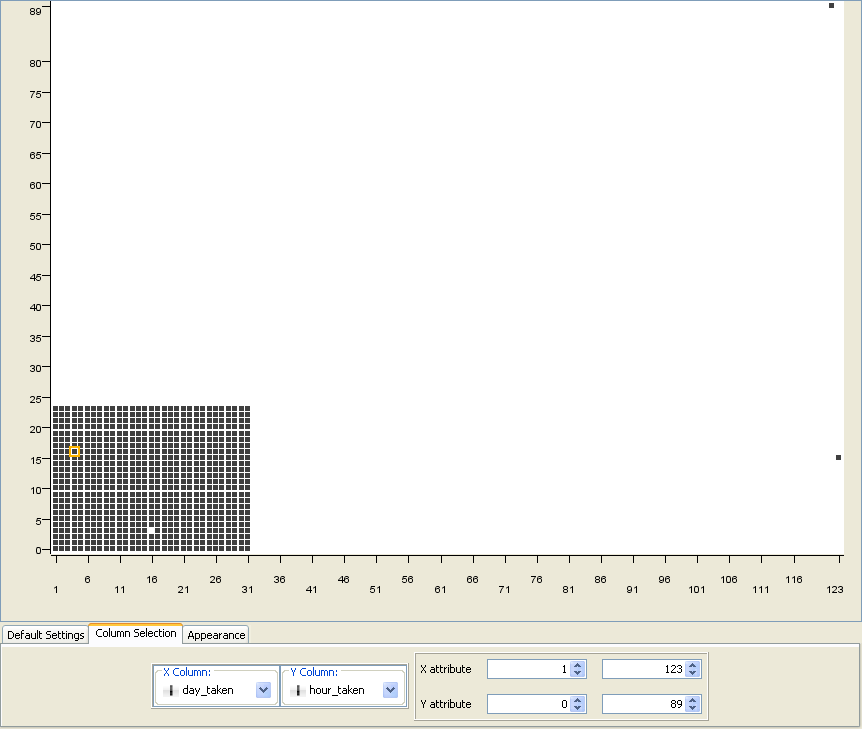
\includegraphics[scale=0.27]{../screenshots/day_hour_before.png}
            \caption{données avant filtrage}
            \label{diagram:day_hour_before}
        \end{figure}

        \begin{figure}[h]
            \centering
            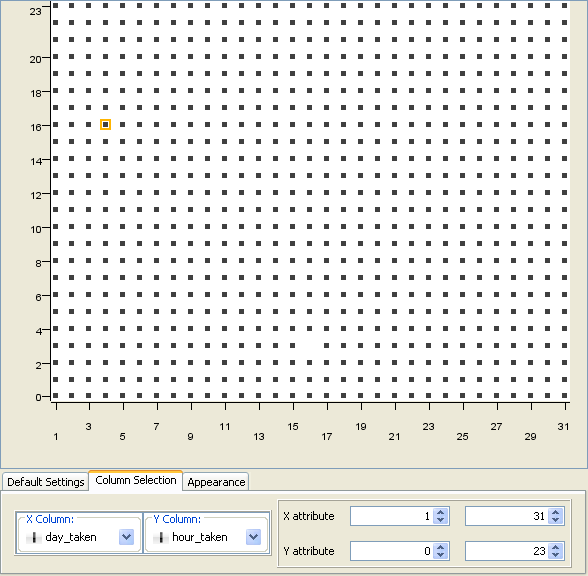
\includegraphics[scale=0.35]{../screenshots/day_hour_after.png}
            \caption{données apr\`es filtrage}
            \label{diagram:day_hour_after}
        \end{figure}

    \pagebreak
    \subsection{Coordonnées GPS}

        Probablement pour des raisons de conversion (ou de troll pur et simple de la part de notre source de données),
        un point était situé aux coordonnées (0, 0). Nous avons donc préféré éliminer ce point individuellement au lieu
        de restreindre les valeurs de latitude et de longitude (de ce fait, nous avons aussi gardés des points éloignés
        du centre de Lyon, mais pertinents dans notre étude)

        \begin{figure}[h]
            \centering
            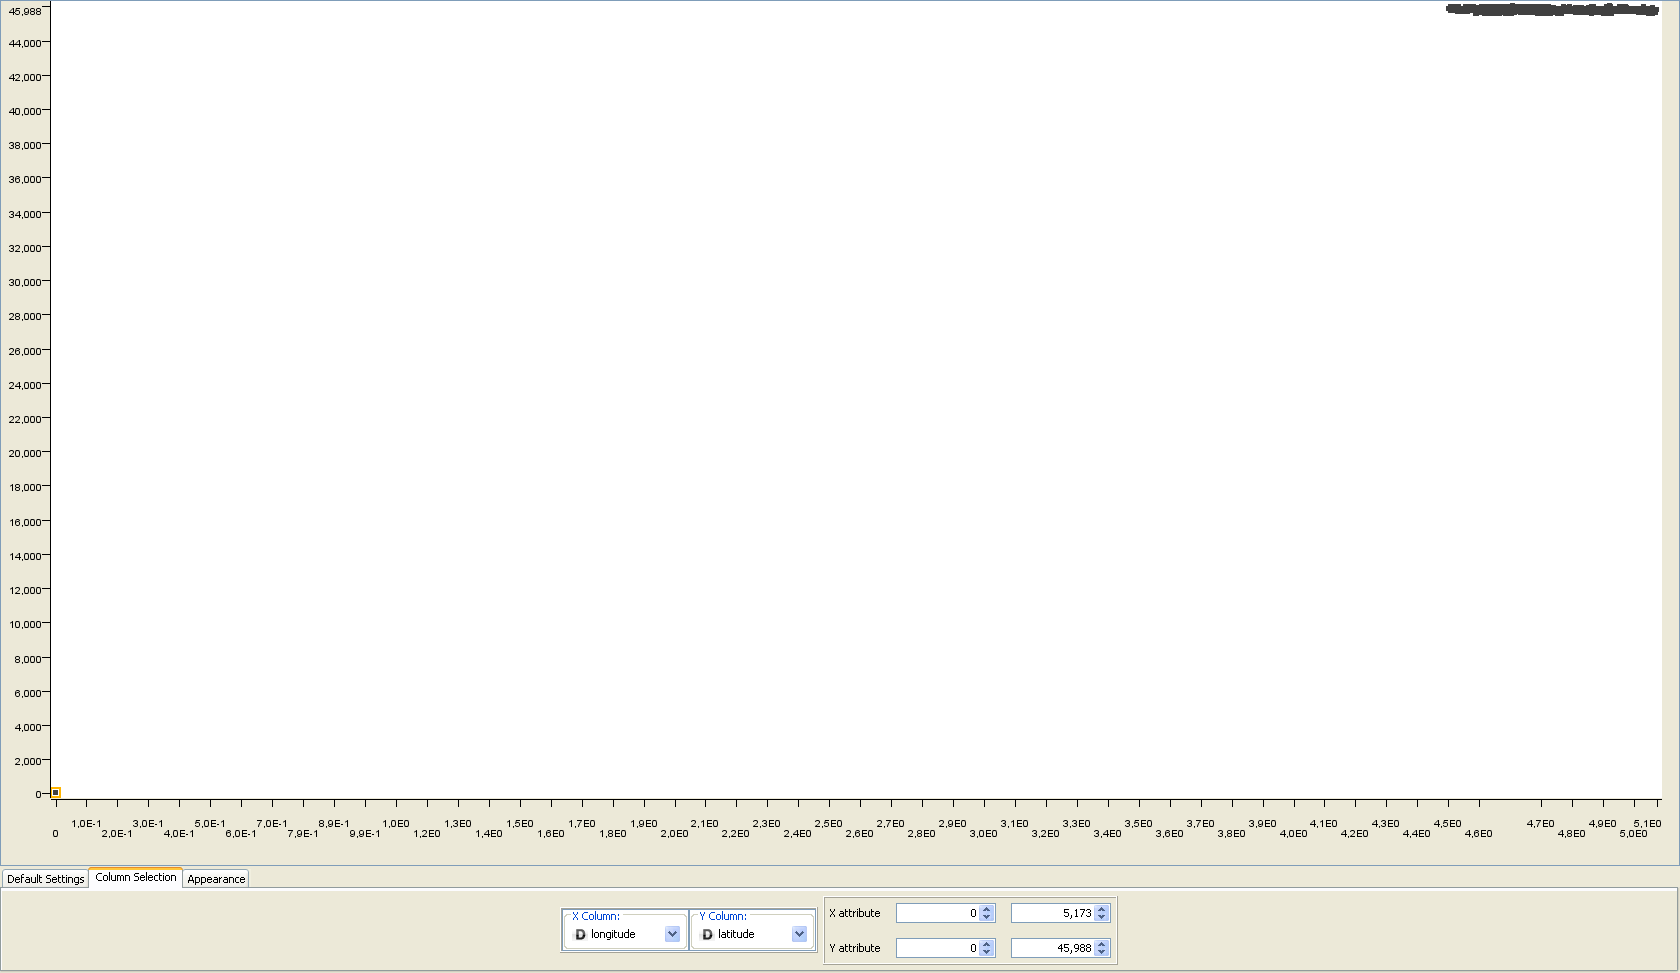
\includegraphics[scale=0.22]{../screenshots/geographic_before.png}
            \caption{Coordonnées GPS avant filtrage}
            \label{diagram:geographic_before}
        \end{figure}

        \begin{figure}[h]
            \centering
            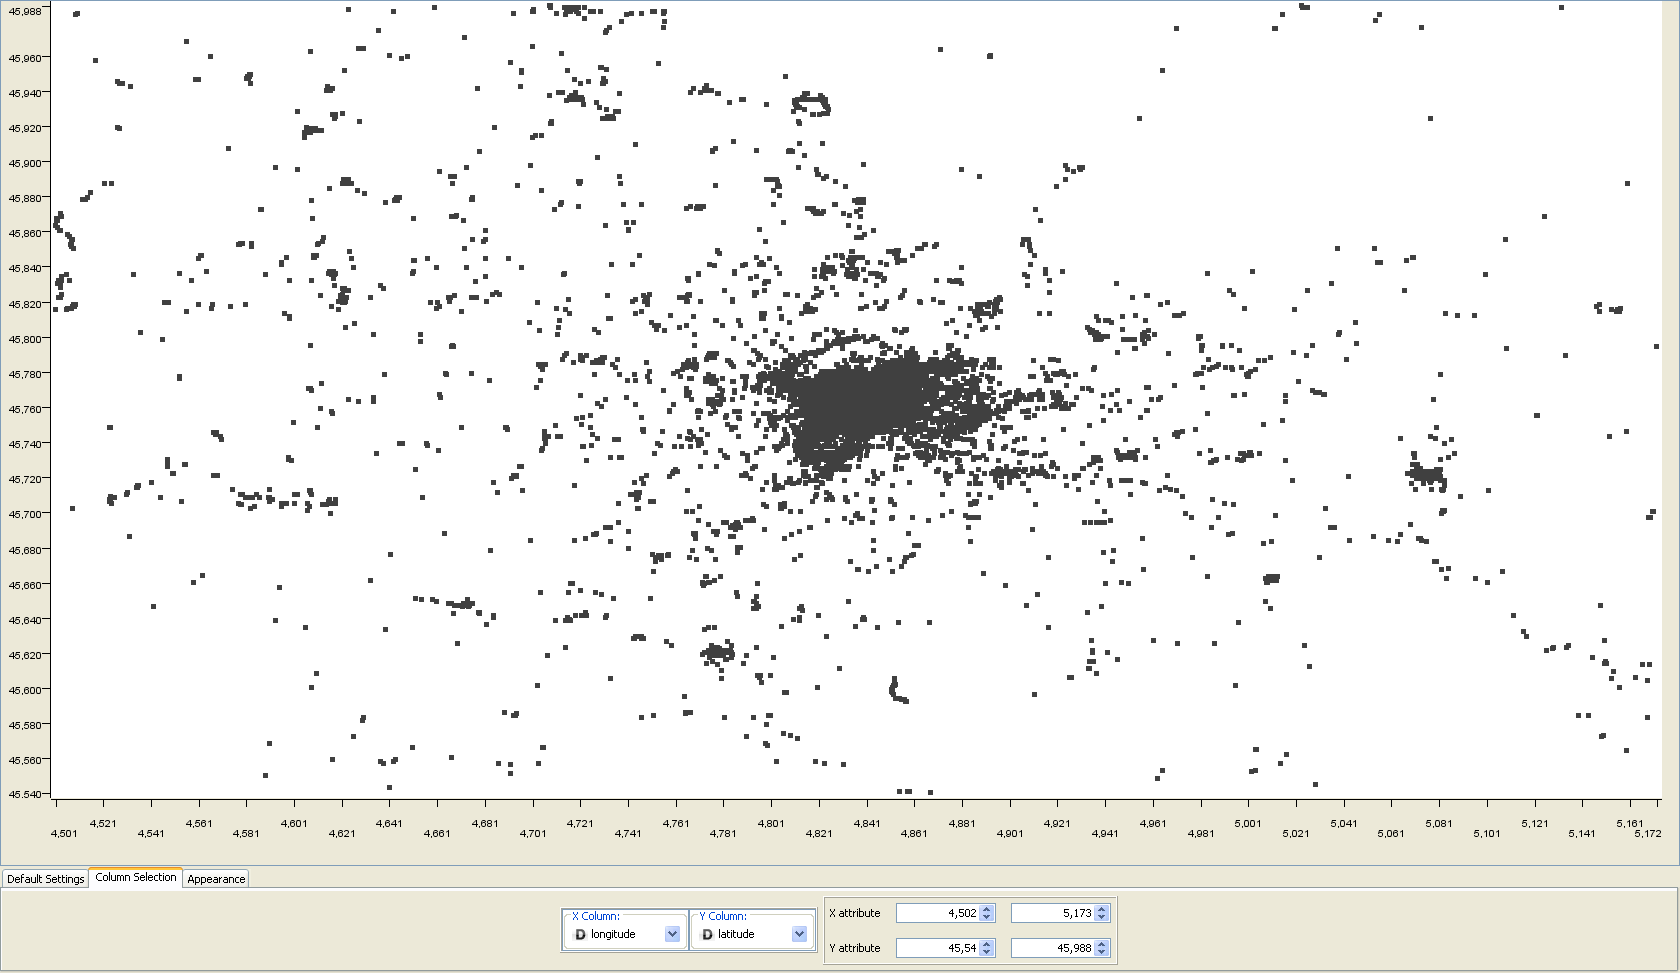
\includegraphics[scale=0.22]{../screenshots/geographic_after.png}
            \caption{Coordonnées GPS apr\`es filtrage}
            \label{diagram:geographic_after}
        \end{figure}

	\chapter{Clustering}

\section{Clustering hiérarchique}
    Cette méthode, bien qu'utile quand on ne connaît pas le nombre de clusters
    attendu, ne passe pas à l'échelle~: son exécution sur la totalité du jeu de
    donnée provoque un dépassement de mémoire.

    Nous avons malgré tout réalisé un échantillonnage aléatoire (de 1,000 lignes)
    de notre jeu de données sur lequel on a effectué un \textit{clustering hiérarchique}
    afin d'avoir une idée sur le nombre de clusters qui pouvaient être extraits.

    \begin{figure}[h]
        \centering
        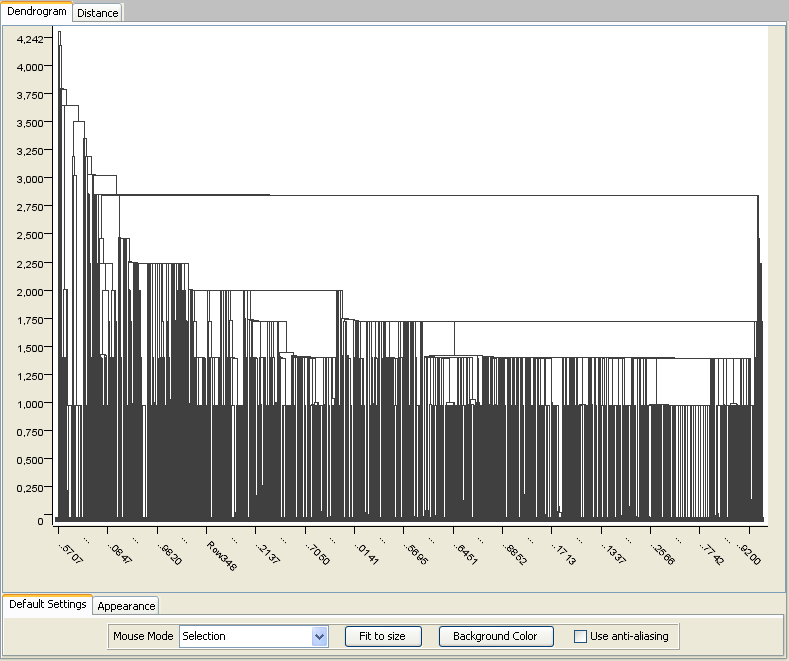
\includegraphics[scale=0.35]{../screenshots/hierarchical_clustering_1000_samples.png}
        \caption{R\'esultat du clusturing hiérarchique sur 1000 \'echantillons}
        \label{diagram:hierarchical_clustering_1000_samples}
    \end{figure}

    Mais même sur un jeu de données aussi restreint (par rapport aux données
    originales), le résultat était difficilement exploitable (car très dense),
    et le fait que les données exploitées représentaient moins de $5\%$ des
    données originales faisait que ce clustering était fort instable (structure
    variant sur des samplings différents).

\section{K-Means}


\section{DBScan}


	%\renewcommand{\chaptermark}[1]{\markboth{\MakeUppercase{#1}}{}}
	%\renewcommand{\sectionmark}[1]{\markright{#1}}

	%\addcontentsline{toc}{part}{Annexes}
	%\part*{Annexes}
	%\appendix
	%\include{implementationExercices}


    % ------------------------------------------------------------------- FOOTER
\end{document}
